% Chapter 2

\chapter{Data Analysis} % Main chapter title

\label{Chapter2} % For referencing the chapter elsewhere, use \ref{Chapter1} 

%----------------------------------------------------------------------------------------

This chapter aims to explain first of all what is the "big data analysis", and why it is important in the modern world. Subsequently it will be exposed the application of bid data analysis in AEgIS experiment, with reference to the used technologies and the choices made.   


\section{What is?}
According to the John Tukey's definition data analysis is: 

"Procedures for analyzing data, techniques for interpreting the results of such procedures, ways of planning the gathering of data to make its analysis easier, more precise or more accurate, and all the machinery and results of (mathematical) statistics which apply to analyzing data" 
( \url{http://projecteuclid.org/euclid.aoms/1177704711} ).

The basic idea is that in the modern world almost each activity can provide a big amount of data, but only a few of them are really useful to gain interesting information. The data analysis is a structured process that allows to select the most important parts of this row data and exploit them to gain information able to answer questions, test hypotheses and approve or disprove theories.
In the following figure (2.1) we can see the schema of this process. 

\begin{figure}[H]
\centering
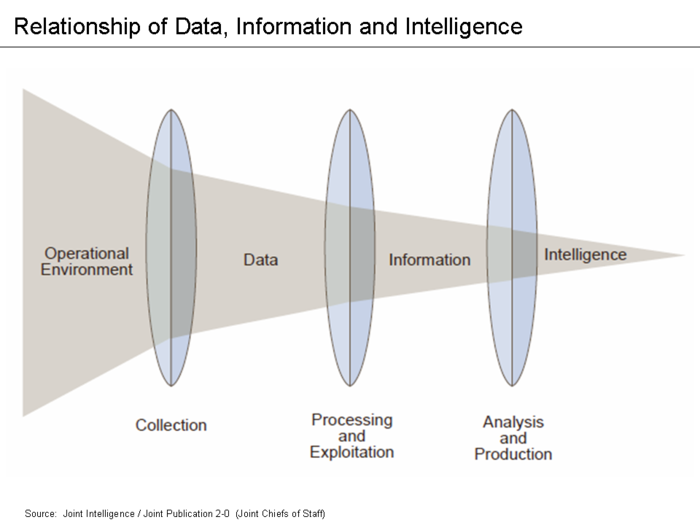
\includegraphics[scale=0.5]{DataAnalysisProcess.png} 
\caption{Here is visible a basic schema of data processes and analysis}
\end{figure}

Data analysis can be divided in some steps:

\begin{enumerate}

% 1
\item Data collection: data can be collected in a variety of ways. For example is possible to collect them using sensors in the environment, such as satellites, recording devices, physical sensors etcetera. It is also possible to obtain data through interviews, downloads from online sources, or reading documentation... so the analysis is feasible with a large variety of kinds and sources of data. 

% 2
\item Data processing: raw data must be well-organized for analysis: for example, placing data into row, columns, vector, etcetera (but the definition of "well-organized" in this context varies according to the kind of analysis to which it is intended).

% 3
\item Data cleaning: Once pre-processed and organized, the data may be incomplete, contain duplicates, or contain errors. Data cleaning is the process of correcting these errors, eliminating duplicates and handling incomplete data. Some ways to do this are record matching (confrontation between the records to find if there is something suspicious), validation of data (if there is the sureness that data values has to respect some limits), overall evaluation of quality of existing data, de-duplication (process used to remove duplicates). For particular kinds of input this process is very complex (for example vocal input needs an advanced spell-checker), for others is simple (for instance online-survey interviews made using closed choices) 

% 4
\item Exploratory data analysis: in this step the data is analyzed. There are a variety of techniques referred to as "exploratory data analysis", they aims to begin understanding the real content of the data. This process may result in Descriptive statistics, such as the calculation of average or median, or in Data visualization, that allows to examine the data in graphical format, through graphics and other graphical objects.

% 5
\item Modeling and algorithms: another step is using mathematical models to find relations between different variables, such as causality or correlation. An example of this process is the regression analysis.

% 6
\item Communication: this is the final step, and it is absolutely not trivial. It is important to find a way to report the obtained information to the user in an understandable format. The communication must be adapted to the different users, in order to let the data analysis able to meet their requirements.

\end{enumerate}

\section{What a user can obtain from the data?}

An user can benefit from the analysis of big data in various ways, in particular a working data analysis software can perform the subsequent tasks:

\begin{enumerate}

% 1
\item Retrieve Value: the system receives in input a group of cases (for instance case-A, case-B etcetera) and a set of variables (for instance variable-A, variable-B etcetera), and produces in output the values that the variables of the set take in the inserted cases (in case-A, case-B, the user is interest in variable-A and variable-B, and the system gives in output variable-A = x and variable-B = y).

% 2 
\item Filter: the system can show only the subset of the data that respects some conditions.

%3
\item Find extremums, ranges and identify data distribution: the system can show the maximums o minimums values in the datasets, and in how large is the range in that the values are distributed. It is also possible to approximate with mathematical functions the statistical distributions of subsets of data. 

%4 
\item Find Anomalies: the system checks the dataset to find if there are some exceptional values, that are source of interest and needs an explanation (errors in the data? unknown phenomena?).

%5
\item Clustering: the analysis is strongly easier if it is possible to group different subset of data with similar characteristics. For example: in a market research, obtaining a correct clusterization of the customer allows to understand the different categories of customers, which have different goals and needs.      

\end{enumerate}

\section{Relevance in the modern market}

The big data analysis in recent years has taken an extraordinary importance, as stated by The Economist, who says:
"Big data has increased the demand of information management specialists in that Software AG, Oracle Corporation, IBM, Microsoft, SAP, EMC, HP and Dell have spent more than 15 billion dollars on software firms specializing in data management and analytics. In 2010, this industry was worth more than 100 billion dollars and was growing at almost 10 percent a year: about twice as fast as the software business as a whole."
(taken from \url{http://www.economist.com/node/15557443}).
This fact shows that companies (and governments) have realized the importance of the exploiting of the huge amount of data that the modern world produce. The hugeness of this amount of raw data is visible in the following data:

"There are 4.6 billion mobile-phone worldwide, and 1-2 billion people accessing the internet. In recent years, more than 1 billion people in the world entered the middle class, which means more people become more literate, which in turn leads to information growth. The capacity to exchange information has grown rapidly in recent years, to 667 exabytes annually in 2014." 
(data taken from: Wikipedia \url{https://en.wikipedia.org/wiki/Big_data#Applications}; The Economist \url{http://www.economist.com/node/15557443}; martinhilbert.net  \url{http://www.martinhilbert.net/WorldInfoCapacity.html/})

An advanced big data analysis offers good opportunities to improve decision-making abilities, whether in a public or private institution, in numerous fields such as health care, employment, economic productivity, resource management etcetera. 

Despite this kind of analysis provides benefits in a wide set of fields, in this document is specially important show the opportunities that data analysis can provide in a scientific environment, in particular in the AEgIS experiment. This is the main topic of the following paragraph.

\section{Data Analysis at CERN}

Some experiments at the CERN represents about 150 million sensors delivering data 40 million times per second. There are nearly 600 million collisions per second. The point is that not all these collisions are scientifically interesting. In the huge amount of collisions discussed previously there are only around 100 collisions of interest per second.
This leads a big problem: it is difficult to find a rational way to work with flows of data having this dimension, and it is absolutely necessary to take only the part of the data actually required for the scientific analysis, but it is also important don't waste nothing interesting in this dataset.

Another problem to solve to meet the user's requirements is related to the speed with which physicists develop and change focus in their experimental work: they are not interested always at the same things, and they cannot predict in advance what they will need in the future, because their needs are related the process of experimentation, and can change continuously. 
So a system of analysis must be very flexible and dynamic, always ready to answer to new requirements, always able to find exactly what is the "interesting" part of data.  

This kind of problems are not just CERN's problems, they are common in major research centers. Bob Jones, Project Leader at CERN, says:
"CERN is a leader but not alone in having to deal with such high data throughputs. We expect to see similar scales in other sciences (such as next generation genome sequencing as well as the Square Kilometre Array which will primarily be deployed in Australia and South Africa) and various business sectors linked to the growing Internet of Things in the near future."
(quote taken from \url{http://www.cloudwatchhub.eu/what-big-data-really-looks-cern-universe-and-everything})
 
Big data analysis can provide an answer to this problems: with an intelligent and parameterizable process of filtering it is possible extract only the subset of scientifically interesting information, and delivering them to the users in an organized and structured way, by tables, statistical values, graphical images. 
In this way is possible improve the productivity of the physicists, exempting them from unnecessary commitments and dynamically meeting their needs. 

COMMENT: %TODO %TODO %TODO %TODO %TODO %TODO %TODO TODOTODOTODO ASCOLTATI QUESTO VIDEO E VEDI SE CI SONO BUONI SPUNTI https://ieondemand.com/presentations/big-data-analytics-for-improving-the-cern-s-large-hadron-collider-operations

\section{Root - Physical Data Analysis }

There are some software (often free software) specialized in the analysis of big data. Each these software has strengths and weaknesses, and none of them appear to be absolutely better than the others. Following there are some examples:
 
\begin{enumerate}

% 1
\item MATLAB (matrix laboratory) is a numerical computing environment. It is a proprietary (so, it is not available for free, and it is quite expensive) programming language developed by MathWorks. Matlab allows matrix manipulations, plotting of functions and data, implementation of algorithms, creation of user interfaces, and interfacing with programs written in other languages, including C, C++, Java, Fortran and Python. 
Some detractors say that the statistical support is incomplete if compared with other solutions (also free).

% 2
\item R is a programming language and a software environment for statistical computing. It is supported by the R Foundation for Statistical Computing.The R language is widely diffused for developing statistical software and for data analysis. His popularity has increased in recent years, this is due to the fact that R is free and provides to user a good front-end interface. On the other hand some users say that the learning curve is quite hard at the beginning (in a big research center this is not a big problem..).  

% 3 
\item SciPy/NumPy/Matplotlib are libraries that work in the field of big data analysis written for the general purpose language Python. It is a quite immature technology, but it is freely available and it uses a general purpose and widely diffused language like Python.

% 4
\item ROOT is an object-oriented program and library developed by Cern, released the first time in 2003 (the process of development started in 1994 and it has been continuously updated until now). It was originally designed for particle physics data analysis and contains several features specific to this field, but it is also used in other applications such as astronomy and data mining. 

\end{enumerate}

For the AEgIS experiment ROOT is the chosen software to carry out the activities of data analysis. The reason is that this software has been specifically tailored to meet the requirements of the analysis applied to particle physics.
Another advantage of Root is that there are a lot of libraries created during the years related to the activities of the experiments of the Cern and it is nearly impossible rebuilt them from scratch with another software.

ROOT development was started by René Brun and Fons Rademakers in 1994 (but a more extended and precise list of collaborators is accessible here \url{https://root.cern.ch/root/htmldoc/guides/users-guide/ROOTUsersGuide.html#preface}). 
The ROOT's user guide start with this prefaction, that explains in detail how ROOT was born.:
"In late 1994, we decided to learn and investigate Object Oriented programming and C++ to better judge the suitability of these relatively new techniques for scientific programming. We knew that there is no better way to learn a new programming environment than to use it to write a program that can solve a real problem. After a few weeks, we had our first histogramming package in C++. A few weeks later we had a rewrite of the same package using the, at that time, very new template features of C++. Again, a few weeks later we had another rewrite of the package without templates since we could only compile the version with templates on one single platform using a specific compiler. Finally, after about four months we had a histogramming package that was faster and more efficient than the well-known FORTRAN based HBOOK histogramming package. This gave us enough confidence in the new technologies to decide to continue the development. Thus was born ROOT."
(Taken from \url{https://root.cern.ch/root/htmldoc/guides/users-guide/ROOTUsersGuide.html#preface})


This software is partially released under GPL (this means that everyone is allowed to use, redistribute and change the software, but any changes made must also be licensed under the GPL), and partially under LGPL (The LGPL is similar to the GPL, but is more designed for software libraries in that the developer wants to allow non-GPL applications to link to your library and utilise it).

ROOT is an object oriented framework that aims to solve problems related to high-energy physics. To better understand what is ROOT is important to start with understanding what is a framework: in IT a framework is a structure that helps the programmers providing them a set of already working utilities and services (for example, I/O, graphics, etcetera) often related to the sector in which the framework aims to work (for example, the services of a web development framework are related to the layout of a web page, to the organization of DBs etcetera). ROOT in particular offers services, functions, and packages related on the world of high-energy physics research, that allow to save much work.
It provides, for example the possibility to use a computer's graphics subsystem and operating system with abstraction, allowing the developer to create a graphical user interface and a GUI builder. Root provides also an abstract platform that allows to run C++ and command line scripts. More precisely Root includes (among others):

\begin{enumerate}

% 1
\item Libraries related to histogramming and graphing, that allows the developer to easily represent graphically statistical distributions. Also 3D visualization is allowed.

% 2
\item Libraries related to regression analysis.

% 3
\item Various statistics tools. 

% 4
\item Libraries related to digital image processing and manipulation.

% 5
\item Libraries aimed to allow parallel computing, (to parallelize data analysis can be really useful in order to manage the complexity of the calculations).

%6
\item The possibility of interfacing in both directions with code written in Python or Ruby.

%7 
\item The possibility of interfacing with Javascript, allowing the developer to access Root functionalities by a Browser.

\end{enumerate}

In the following figure (2.2) we can see the structure of the ROOT's libraries:

\begin{figure}[H]
\centering
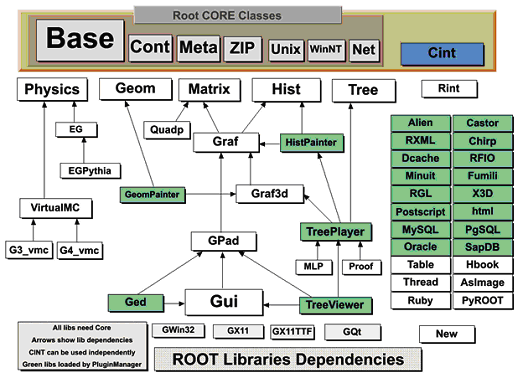
\includegraphics[scale=0.5]{RootStructure.png} 
\caption{ROOT structure}
\end{figure}


